\section{Background}
\label{background}
In this section we give an overview of prior work 
and the context of this research.

\subsection{Reactive Programming}
\label{nutshell}
Reactive Programming (RP) is a declarative programming paradigm for working with streams of input data. 
According to the original definition\footnote{
``Reactive programs [..] maintain a continuous interaction with their environment, at a speed which is determined by the environment, not the program itself.''~\cite{berry1989real}
} a reactive program must interact with the environment `at a speed which is determined by the environment'.
This means that when a reactive program is run it sets up the data pipeline declared in the code and waits until input arrives c.q. the environment changes.
Reactive Programming languages and libraries provide developers with the appropriate abstractions and methods to create such programs.

The programming paradigm of Reactive Programming is implemented by multiple languages and libraries. Many RP implementations share a notion of a collection that abstracts over \textit{time}, in contrast to \textit{space} like standard collections, be it \textit{Observable} (Rx~\cite{meijer2010subject}), Signal (Elm~\cite{czaplicki2012elm}), Signal/Event (REScala~\cite{salvaneschi2014rescala}) or Behavior/Event (FRP~\cite{elliott1997functional}). In this paper we focus on the Rx formulation, but our work is applicable to other RP implementations to some extend. 

Understanding how we, given the Rx language, arrive at our visualization requires at least minimal understanding of Rx.
Rx introduces two types \textit{Observable} and \textit{Observer}, derived by dualizing the Iterable and Iterator types. Observables define the data flow and Observers receive the data, possibly moving the data further down the stream. Figure \ref{sample1} shows a very basic example of a in situ data flow in Rx. First an Observable is created, here using the static \code{of} method, then dependent Observables are created using the \code{map} and \code{filter} methods on the Observable instance. Finally we \code{subscribe} to start the data flow and send the data in the flow to the console (eg. JavaScript's stdout).

\begin{figure}

\begin{subfigure}[a]{\columnwidth}
\inputminted[tabsize=2]{javascript}{listings/sample1.js}	
\caption{Rx code example}
\label{sample1}
\end{subfigure}

\begin{subfigure}[b]{\columnwidth}
\centering
\begin{tikzpicture}[->,>=stealth',shorten >=1pt,auto,node
    distance=2.8cm,
                    semithick,scale=0.8, every node/.style={scale=0.8}]
    \tikzstyle{every state}=[]

    \node[state] (A) {$ o_1 $}; \node[state] (B) [right of=A] {$ o_2 $};
    \node[state] (C) [right of=B] {$ o_3 $};

    \node[state] (X) [below right =1cm of A] {$ s_3 $}; \node[state] (Y)
    [right of=X] {$ s_2 $}; \node[state] (Z) [right of=Y] {$ s_1 $};

    \path (B) edge node {source} (A) (C) edge node {source} (B) (A) edge
    [bend left] node {map(\_ * 2)} (B) (B) edge [bend left] node {filter
    (\_ < 3)} (C) (X) edge node[below] {destination} (Y) (Y) edge node[below]
    {destination} (Z) (Z) edge node {subscribe} (C) (Y) edge node {subscribe}
    (B) (X) edge node {subscribe} (A);

    \draw[<-] (A) -- node[above] {of(1,2,3)} ++(-2cm,0);
    %\draw[<-] (Z) -- node[below] {subscribe} ++(2cm,0);

\end{tikzpicture}

\caption{Rx graph example}
\label{chaincreate}
\end{subfigure}

\caption{Basic Rx  Observables}

\end{figure}

It is important to note that Observables are lazy, they are the blueprint of a data flow. Only when the \code{subscribe} method of Observable is called the data flow is created by recursively subscribing up the stream. \textit{Observer}s are subscribed to each Observable until the source Observables are reached which then are setup and can start emitting the data.
This is illustrated in figure \ref{chaincreate}. Here $o_1$, $o_2$ and $o_3$ represent Observables defined in Figure \ref{sample1}. Inside the \code{subscribe} call $s_1$ is created and passed to $o_3$, which in turn will recursively subscribe to $o_2$ with a new Observer $s_2$ with destination $s_1$, until the full chain is subscribed.
The origin of this design is the duality between Observables and \textit{Iterables} - as first described by Meijer~\cite{meijer2010subject}, where Observers are dual to \textit{Iterators}.

\begin{figure}

\begin{subfigure}[a]{\columnwidth}
\inputminted[tabsize=2]{javascript}{listings/sample3.js}	
\caption{Higher order flatMap operation}
\label{sample3}
\end{subfigure}

\begin{subfigure}[b]{\columnwidth}
\centering
\begin{tikzpicture}[->,>=stealth',shorten >=1pt,auto,node
    distance=2.8cm,
                    semithick,scale=0.8, every node/.style={scale=0.8}]
    \tikzstyle{every state}=[]

    \node[state] (A) {$ o_2 $}; \node[state] (B) [right of=A] {$ o_3 $};
    \node[state] (C) [right of=B] {$ o_4 $};

    \node[state] (X) [below right =1cm of A] {$ s_3 $}; \node[state] (Y)
    [right of=X] {$ s_2 $}; \node[state] (Z) [right of=Y] {$ s_1 $};

    \node[state] (F) [below =2cm of B] {$ o_1 $}; \node[state] (P) [below
    =1.8cm of Y] {$ s_{4,n} $}; \node[state] (Q) [below =0.3cm of P] {$
    s_{4,m} $};

    \path (B) edge node {source} (A) (C) edge node {source} (B) (A) edge
    [bend left] node {skip(1)} (B) (B) edge [bend left] node {flatMap(()
    => inner)} (C) (X) edge node[below] {destination} (Y) (Y) edge node[below]
    {destination} (Z) (Z) edge node {subscribe} (C) (Y) edge node {subscribe}
    (B) (X) edge node {subscribe} (A)

    (P) edge [bend right] node[sloped,above] {subscribe} (F) (P) edge
    node[sloped,below] {destination} (Z) (Q) edge [bend left] node[sloped,above]
    {subscribe} (F) (Q) edge node[sloped,below] {destination} (Z);

    %  \node[draw=none] (K) at ($ (P) + (-4:-3) $){$\cdots$};
    %  \node[draw=none] (M) at ($ (Q) + (-4:-3) $){$\cdots$};

    % https://tex.stackexchange.com/questions/75497/automata-container-box
    \node [draw=red, label={\color{red}inner}, fit=(F) (P) (Q), inner
    sep=0.5cm,dashed, ultra thick, fill=red!10, fill opacity=0.2] {};
    %\node [draw=blue, fit= (G) (Q) (M), inner sep=0.5cm,dashed, ultra thick, fill=blue!10, fill opacity=0.2] {};

    % https://tex.stackexchange.com/questions/160643/ellipsis
    \draw[<-] (A) -- node[above] {of(1,2,3)} ++(-2cm,0); \draw[->] (F)
    -- node[above] {$ \cdots $} ++(-2cm,0); \draw[<-] (P) -- node[above]
    {$ \cdots $} ++(-3cm,0); \draw[<-] (Q) -- node[above] {$ \cdots $}
    ++(-3cm,0);

\end{tikzpicture}

\caption{Higher order visualization}
\label{chainhigher}
\end{subfigure}

\caption{Higher order Observables}

\end{figure}

More complex programs feature operators that merge Observables, split Observables or handles higher order Observables, resulting in more complex graphs. While merging and splitting happens on an Observable level (the \code{source} property still points to the dependency) higher order Observable flattening manifests only in Observer structure, as shown in Figure \ref{chainhigher}.

Creating the Observable we will call the \textit{assembly} phase, the phase where the subscribe happens the \textit{subscription} phase and data flows in the \textit{runtime} phase. The three phases can be interleaved for different streams, for example when dealing with higher order Observables,  meaning one could use Observables as values inside the data flow. The Observables used as values have yet to start the second phase while the outer stream is in the runtime phase.


\subsubsection{Marble Diagram}
\label{marblediagram}
The term \textit{Marble Diagram} comes from the shape of the glyps in the images used to explain Rx in the official documentation. 
The diagrams contain one or more timelines containing the events that enter and leave Observables. 
Developers can see from the diagram how operators work by inspecting the difference between the timelines, 
where events might be skipped, added, transformed or delayed. 
Mapping time on the x-axis provides insight that is missing when inspecting only a single time slice, like with traditional debuggers.

\begin{figure}[ht]
\centering
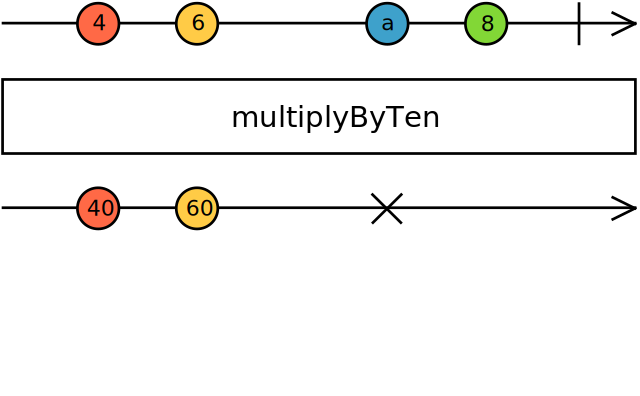
\includegraphics[width=\columnwidth]{images/marble-diagram.pdf}
\caption{Marble Diagram}
\label{marblediagram-image}
\end{figure}

\subsection{Debugging}
Debugging for general purpose languages revolves around 
attaching a debugger, 
stepping through the code, 
attaching code or data breakpoints, 
navigating along different calls in the call stack and 
examining variables and results of expressions~\cite{Spinellis2017}.
Existing research measuring how these different tasks are part of the developers work day found that 
while developers spend much time on comprehending code they do not spend much time inside the debugger~\cite{minelli2015know}.
Beller et al.~\cite{beller2017behavior} found that only 23\% of their subjects actively use the debugger,
with the most common action being adding breakpoints, followed by stepping through code.
The automated tooling of these studies did not measure different kinds of debugging other than using the IDE provided tools, 
however Beller's survey indicates that 71\% also uses printf statements for debugging.  
No indication was given of the language and libraries used by the subjects in the study, 
but the observation that printf debugging is common matches our experience with debugging reactive programs.

% What comprises debugging?
% \item Maybe Zeller / Spinellis?

% \item Petrillo, ``Towards Understanding..." e.g. Swarm debugging
% \item Minelli (know what you did last summer)
% \item Moritz (watchdog 2.0)

\subsection{Debugging for Program Comprehension}
Both debugging and comprehension are processes in the work of programmers.
Initially comprehension was seen as a distinct step programmers had to make
prior to being able to debug programs~\cite{katz1987debugging}, 
but this distinction is criticized by Gilmore saying we must view 
``debugging as a design activity''~\cite{gilmore1991models}, 
part of creating and comprehending programs. 
Maalej et al.~\cite{Maalej2014} interviewed professional developers 
and found that developers require runtime information to understand a program,
and that debugging is frequently used to gather this runtime information.
This supports our view that `debugging' is not only used for fault localization,
but also for comprehension.

% \item Katz, distinct step
% \item Gilmore, comprehension + debugging == linked
% \item Maalej: professionals, avoid deep comprehension, sharing knowlegde

